\section{Large Scale Image Reconstruction for the MeerKAT Telescope} \label{intro}
Image reconstruction on the large scale

Compressed Sensing reconstruction for incomplete measurements.

Large scale image reconstruction applied to data from the MeerKAT Telescope.

\begin{equation}\label{intro:measurement}
V(u, v) = \int\int x(x, y) e^{2 \pi i (ux+vy)} \: dx \: dy 
\end{equation}

sampling pattern is defined by the instrument, in MeerKAT's case the sampling Visibilities are:
\begin{enumerate}
	\item Not Uniform: Pockets of dense samples.
	\item Incomplete: Information for the Image Reconstruction was not measured by the instrument
\end{enumerate}


\subsection{The Major Cycle Architecture}
Algorithms in Radio Astronomy employ the major cycle architecture. The figure shows the major cycle framework. In a major cycle consists of two parts: The non-uniform FFT and an optimization algorithm. 

The non-uniform FFT is responsible for approximating a regularly spaced image from the measurements, and for approximating the measurements corresponding to an image. Non-uniform FFT's are fast approximation algorithms, but by being approximation algorithms, they introduce errors. 

\begin{wrapfigure}{r}{0.6\textwidth}
	\centering
	\vspace{-10pt}
	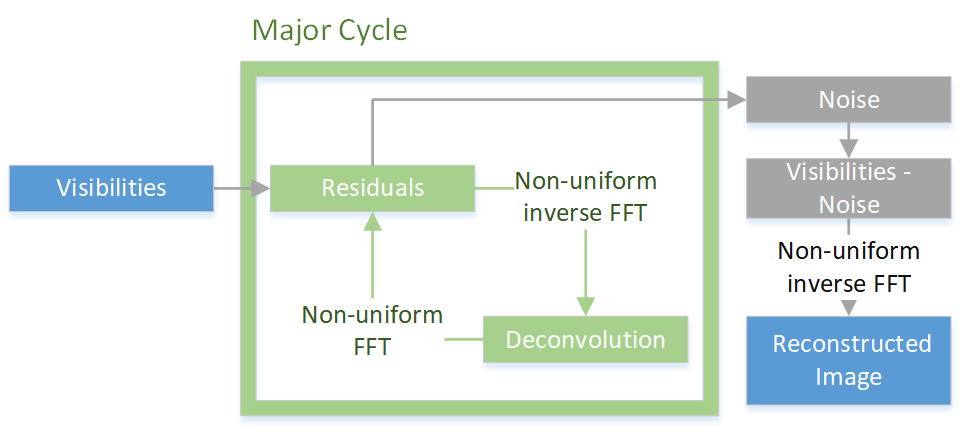
\includegraphics[width=1.0\linewidth]{./chapters/01.intro/Major-Minor.png}
	\caption{The Major Cycle Framework}
	\label{intro:major}
	\vspace{-10pt}
\end{wrapfigure}

A optimization algorithm uses the image and removes the effect of incomplete samples. In the past, CLEAN algorithms were used to remove the effects. For the future, algorithms based on the theory of compressed sensing show promises in image quality.

A full major cycle consists of the following operations: First, it approximates the regularly spaced the regularly spaced image from the measurements. Then the optimization algorithm removes the effects of Incomplete measurements and returns the corresponding image. The major cycle then approximates the measurements corresponding to the image with the non-uniform FFT. The residual measurements are used in the next Major Cycle. In each cycle, two errors get simultaneously reduced:

\begin{enumerate}
	\item The Error introduced by the non-uniform FFT.
	\item The Error introduced by the incomplete measurements.
\end{enumerate}

After several major cycles the algorithm converges on a regularly spaced image which has a small error from non-uniform samples, and a small error from incomplete measurements.

For the optimization algorithm, the CLEAN class of algorithms get used. But algorithms based on the theory of compressed sensing have been shown to produce superior images.


\subsection{Compressed Sensing Reconstructions}
 However, compressed Sensing algorithms come with the drawback of requiring more major cycles.

Current Compressed Sensing reconstructions reduce the number of major cycles. However, the question is if Compressed Sensing can use a different architecture, and scale better to problems of the size of MeerKAT.

There are ways to get rid of the major cycle, but overall the complexity could not be reduced.










